\section{Introduction}

\IEEEPARstart{H}{ow} can we distinguish between two individuals without reasonable doubt? This question has motivated biometric researchers for centuries --- from the pioneer works of Bertillon and Galton
% 's theory of fingerprints and physiognomy 
to recent advances in biometric-enabled mobile payments and wearable devices.
% present in smart clothing and wrist bands. 
Numerous biometric characteristics emerged, and sometimes faded away, as the field progressed, but one biometric trait that has surely withstood the test of time is iris recognition. The iris pattern is unique and ``determined epigenetically by random events in the morphogenesis of this tissue'' \cite{Daugman_PRS_2001}, and thus offers high discrimination power, making it useful in distinguishing even identical twins~\cite{Bowyer_BTAS_2016}.

The recognition power and matching speed of iris recognition has propelled it into use in large-scale applications, \eg Unique ID in India~\cite{UIDAI,Daugman:SPIE:2014}, and the NEXUS system operated jointly by the Canada Border Services Agency and the U.S. Customs and Border Protection to speed up the identification of pre-screened travelers \cite{NEXUS_URL}. As iris recognition becomes more pervasive, the number and variety of attempted attacks naturally intensify, and the problem of \emph{presentation attack detection} (PAD) becomes an essential research topic.

According to the standardized vocabulary in ISO/IEC 30107-1, a \emph{presentation attack} is a ``presentation to the biometric data capture subsystem with the goal of interfering with the operation of the biometric system'' \cite{ISO_30107-1_2016}. An impostor may seek to obtain unauthorized access to an authentication system by \emph{impersonating} a legitimate user, or may want to intentionally \emph{conceal} his or her identity to avoid recognition. Presentation attacks can be realized in various ways, in particular by presenting artifacts, such as paper printouts or textured contact lenses, non-conformant use of a biometric sensor, or even presenting cadaver eyes to the sensor. In this paper, we focus on attacks related to presentation of artificial objects.
%
\begin{figure}[!tb]
    \centering
    \begin{subfigure}[b]{0.99\linewidth}
        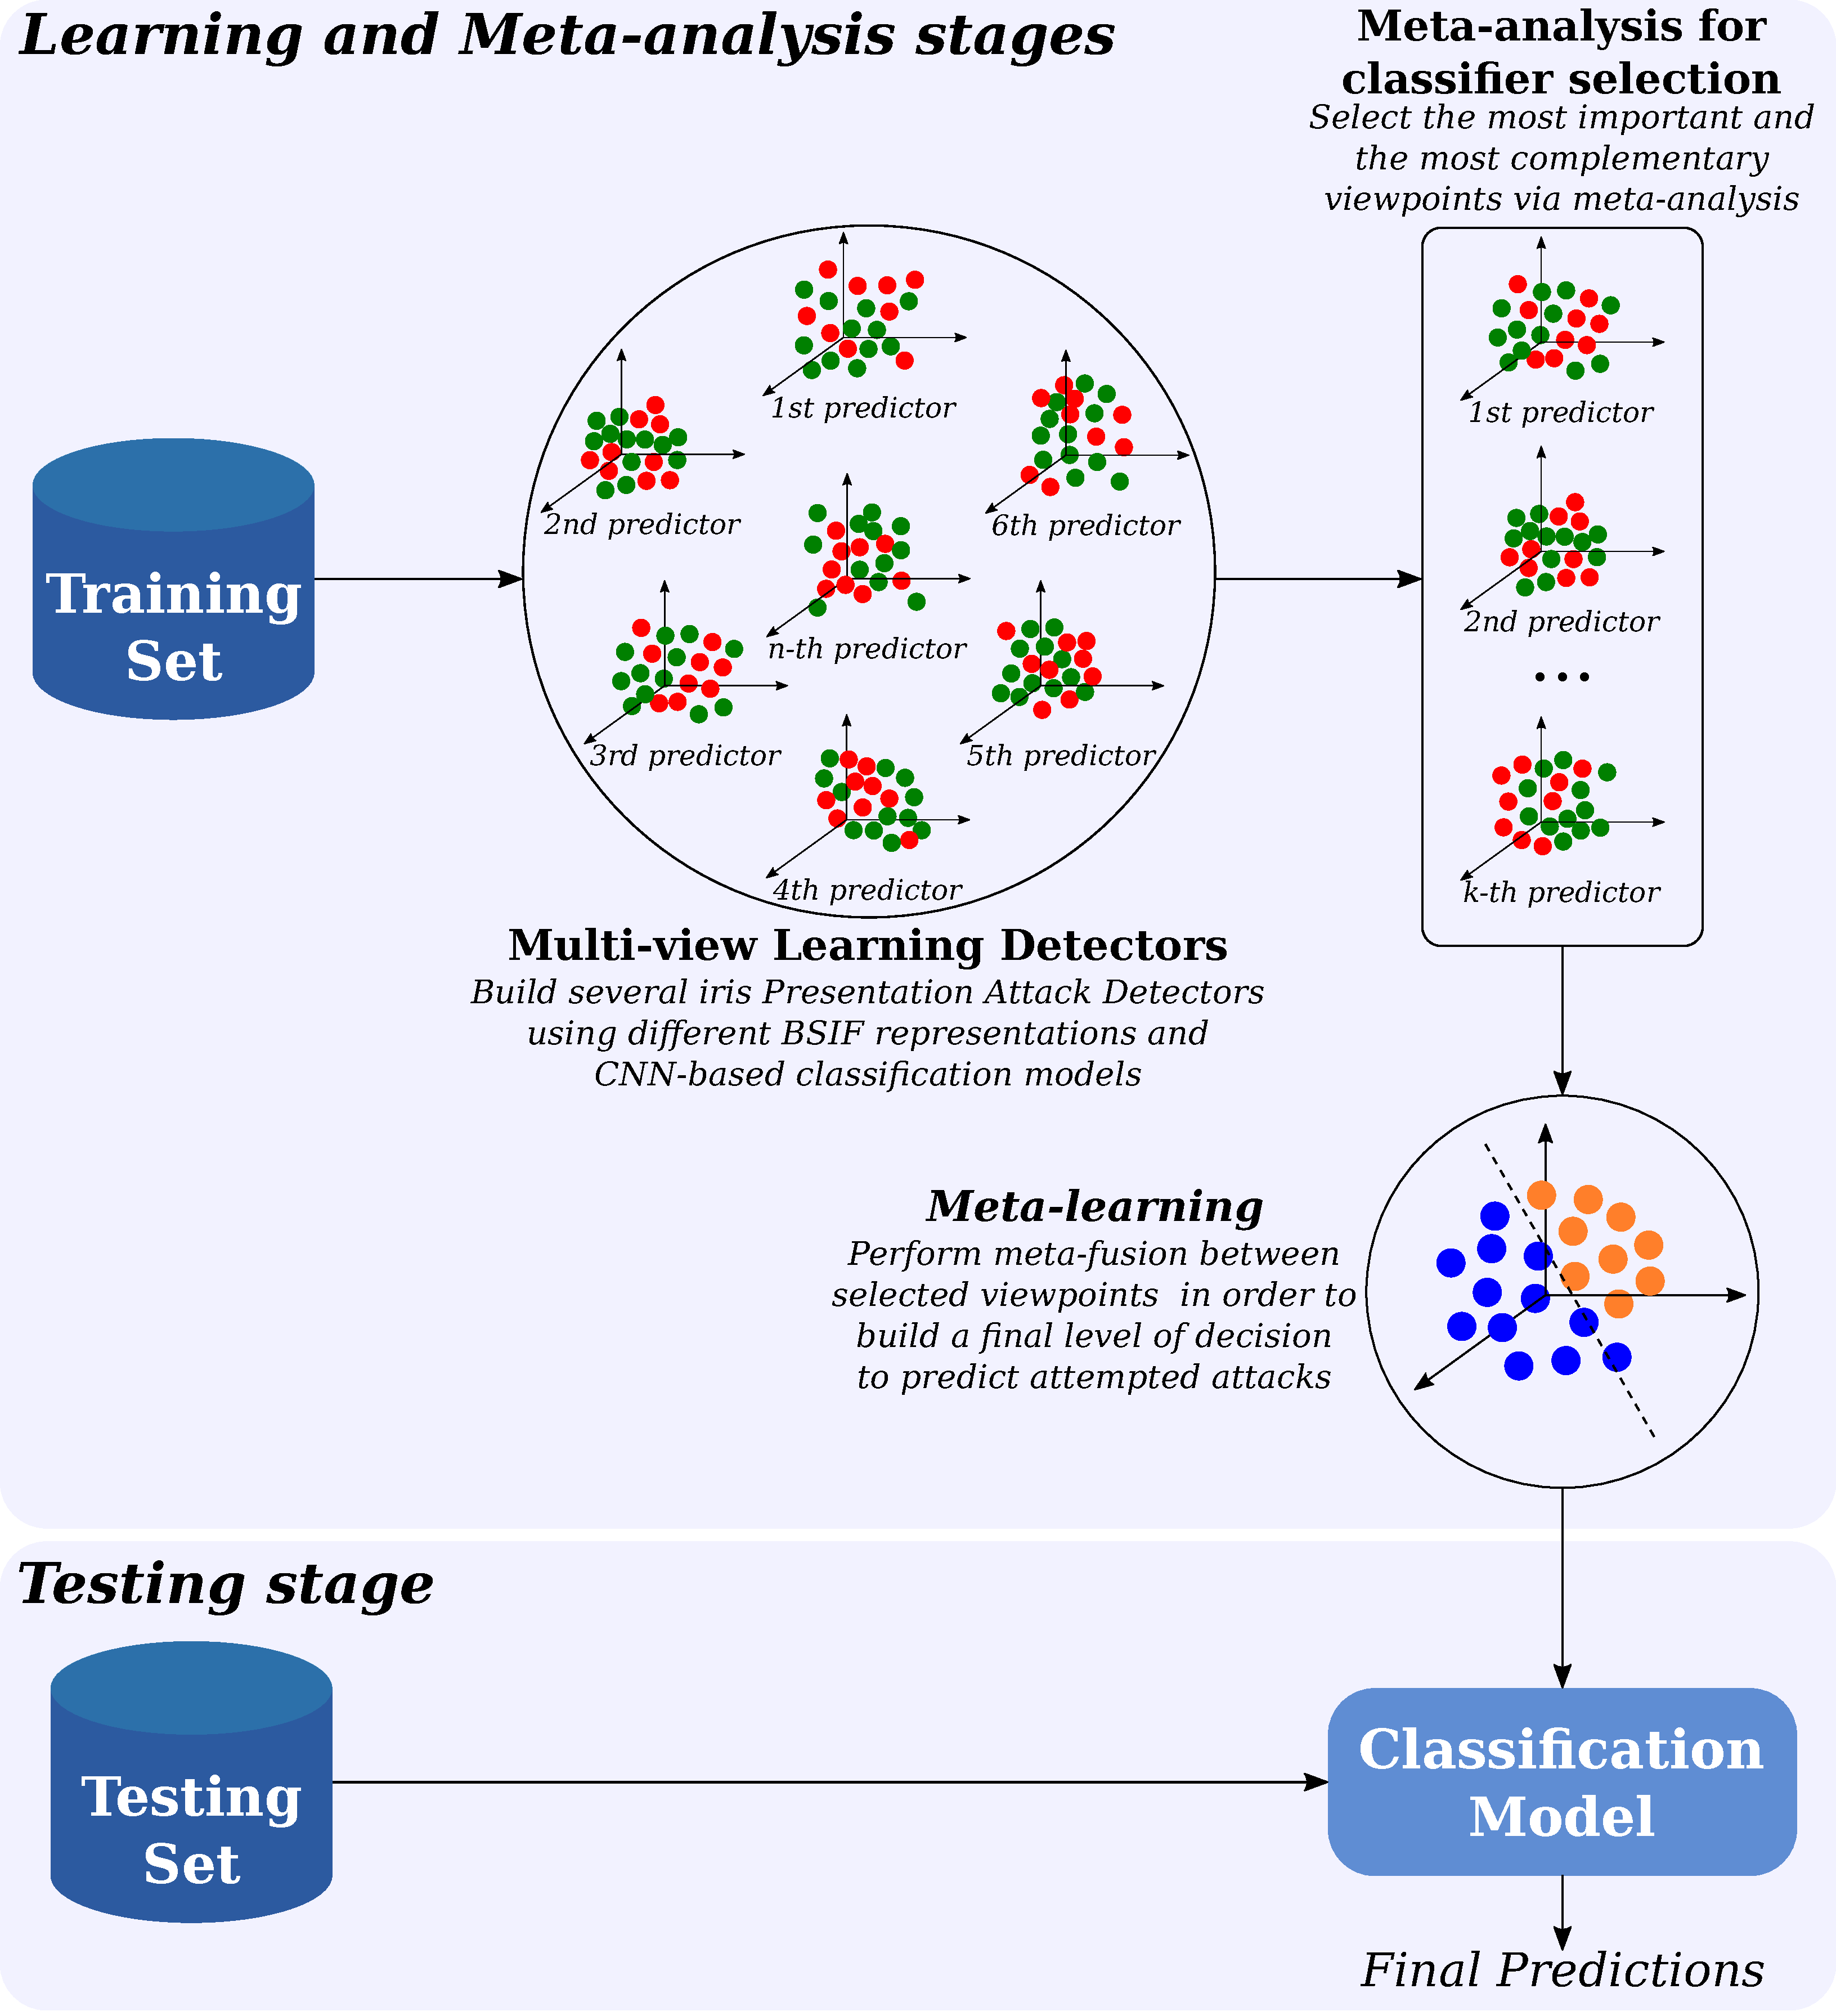
\includegraphics[width=\linewidth]{graphics/method-overview-v4.pdf}
    \end{subfigure}
    \caption{Overview of the proposed method. The first step is generating multiple views from dataset by training lightweight CNNs fed with different BSIF representations, referred to as multi-view-CNN predictors. Next, we select the most promising predictors according to their relevance and complementarity, and combine them via meta-fusion approach. 
    %~\todo[inline]{Maybe we could move this Figure to the first page, to take advantage of it as a graphical abstract.}
    }
    \label{fig:method_overview}
\end{figure}


The Iris Liveness Detection Competition (LivDet-Iris, \url{www.livdet.org})
was begun in 2013.
The third and the most recent edition took place in 2017~\cite{Yambay2017}.
This competition is focused on properly measuring how well current technology withstands presentation attacks employing artifacts.
The sequence of competitions provides an important insight into 
the pace of evolution of iris PAD methods. 
The results reported in the 2017 competition show that iris PAD algorithms are still far from achieving acceptable detection rates. Moreover, the LivDet 2017 results suggest that challenging evaluation protocols, such as cross-dataset and cross-sensor setups --- hereinafter referred to as cross-domain --- can be considered the major limitation of current PAD algorithms and a current open research problem.

In the face of the evident need for better iris PAD,
% of more secure iris recognition systems against presentation attacks, 
this paper introduces a new technique based on exploiting multiple transformations of the input data so as to enhance complementary patterns, leading to a more discriminant manifold separating genuine authentication attempts from attacks.
The multiple transformations are obtained through the combination of hand-crafted and data-driven approaches. While Binarized Statistical Image Features (BSIF)~\cite{Kannala_ICPR_2012} is a popular, effective and partially hand-crafted texture descriptor, Convolutional Neural Networks (CNN) complement the repertoire with powerful description methods capable of learning even the subtlest discrimination clue present in the available training data through a series of non-linear transformations on the input data. 

Although BSIF- and CNN-based methods have been used before in iris PAD, to our knowledge there are no published papers dealing with the challenges of cross-domain deployments, or exploiting complementary properties of various feature extractors and classification strategies when defining a discriminative manifold for the problem under cross-domain constraints. In this vein, we introduce a way of combining both methodologies, hand-crafted and data-driven, in order to offer an iris PAD algorithm that better generalizes to unknown attack types. In addition, we also present a novel meta-analysis algorithm for selecting and aggregating the most prominent data views (\ie transformations), based on two well-known techniques for feature selection: the random forest importance feature weighting and the inter-rater agreement measures, so as to provide the most accurate detection method with the least possible computational impact. Fig~\ref{fig:method_overview} gives an overview of the proposed method.

In summary, the main contributions and novelties of this work are:
\begin{itemize}
    \item{A new approach that leverages multiple pre-trained BSIF filters to effectively train lightweight CNNs;}
    \item{A new fusion algorithm that selects and combines multiple classifiers, considering their importance and complementarity;}
    \item{A thorough cross-domain evaluation of the problem on datasets currently used to document the state of the art in the field;}
    \item{A new PAD method that outperforms the winner of the most recent LivDet-Iris competition, the authoritative international challenge on the subject.}
\end{itemize}

To encourage reproducibility, the source code of our implementation will be publicly available on GitHub. The datasets are already available through the LivDet competition. In the remainder of this paper, we briefly survey important iris PAD methods in prior art (Sec.~\ref{sec:related_work}) and introduce the proposed methodology (Sec.~\ref{sec:proposed_method}). Then we present experiments and validation (Sec.~\ref{sec:experimental_results}) and, finally, draw conclusions and present possible future work (Sec.~\ref{sec:conclusions}).

